\section{Results and Discussion}

\subsection{Results}
The design process yielded the final assembly design in Figures \ref{fig:final3D} and \ref{fig:finalassembly}. The fabrication process on the other hand yielded the assembled mobile platform in Figure \ref{fig:fabassemblywithtop} and Figure \ref{fig:fabassemblyplatform}.


\begin{figure}[H]
    \centering
    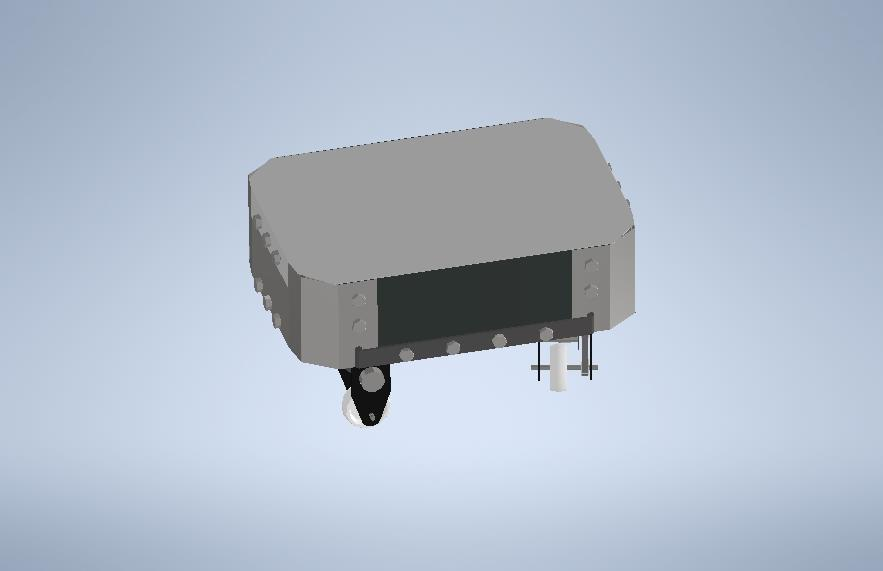
\includegraphics[scale = 0.6]{Figures/final3D.jpg}
    \caption{3D Design}
    \label{fig:final3D}
\end{figure}

\begin{figure}[H]
    \centering
    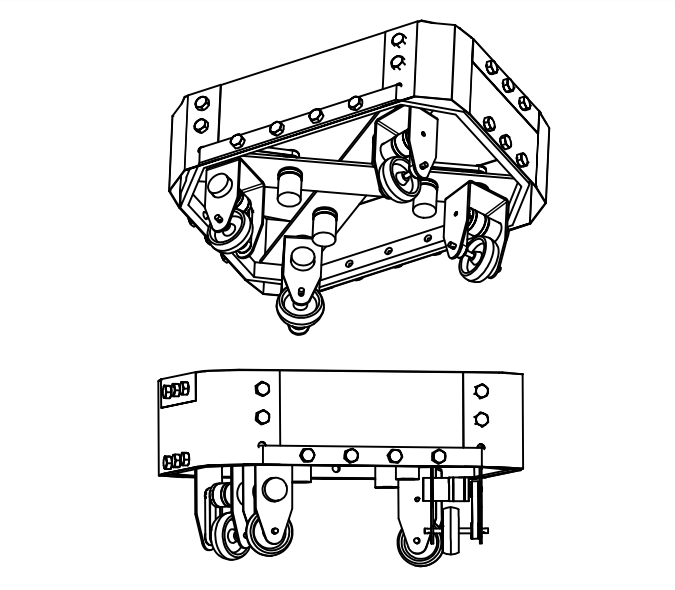
\includegraphics[scale = 0.8]{Figures/NewFinalDesignDWG.png}
    \caption{Assembly Drawing}
    \label{fig:finalassembly}
\end{figure}

\begin{figure}[H]
    \centering
    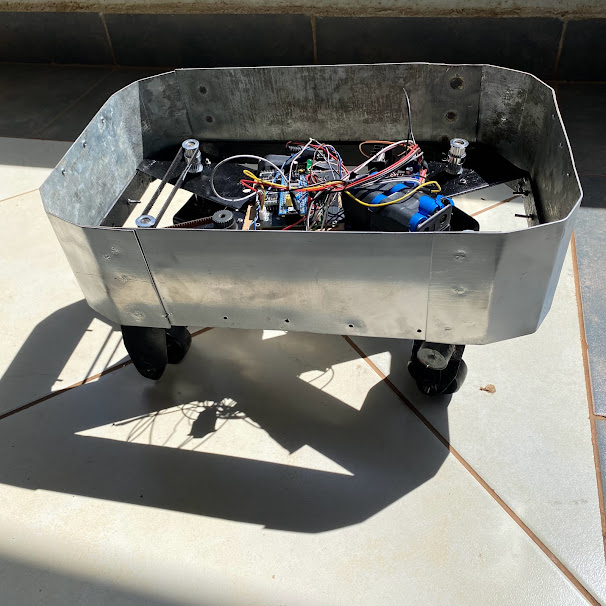
\includegraphics[scale = 0.4]{Figures/finalAssemblyOPEN4.jpg}
    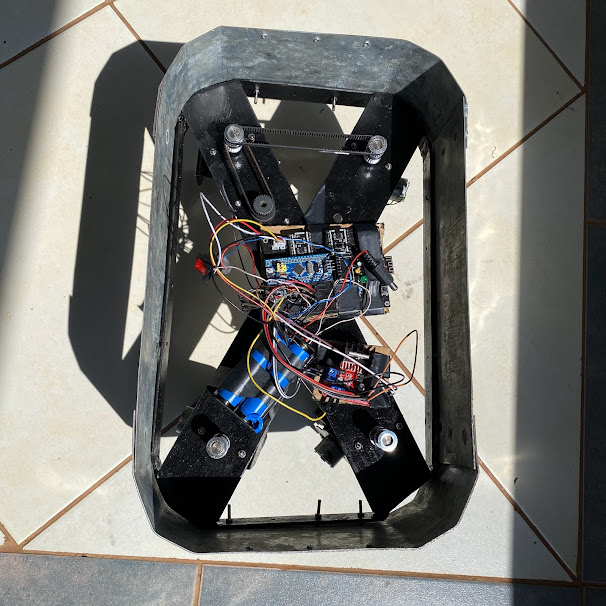
\includegraphics[scale = 0.4]{Figures/finalAssemblyOPEN3.jpg}
    \caption{Fabricated Assembly with Open Top}
    \label{fig:fabassemblywithtop}
\end{figure}

\begin{figure}[H]
    \centering
    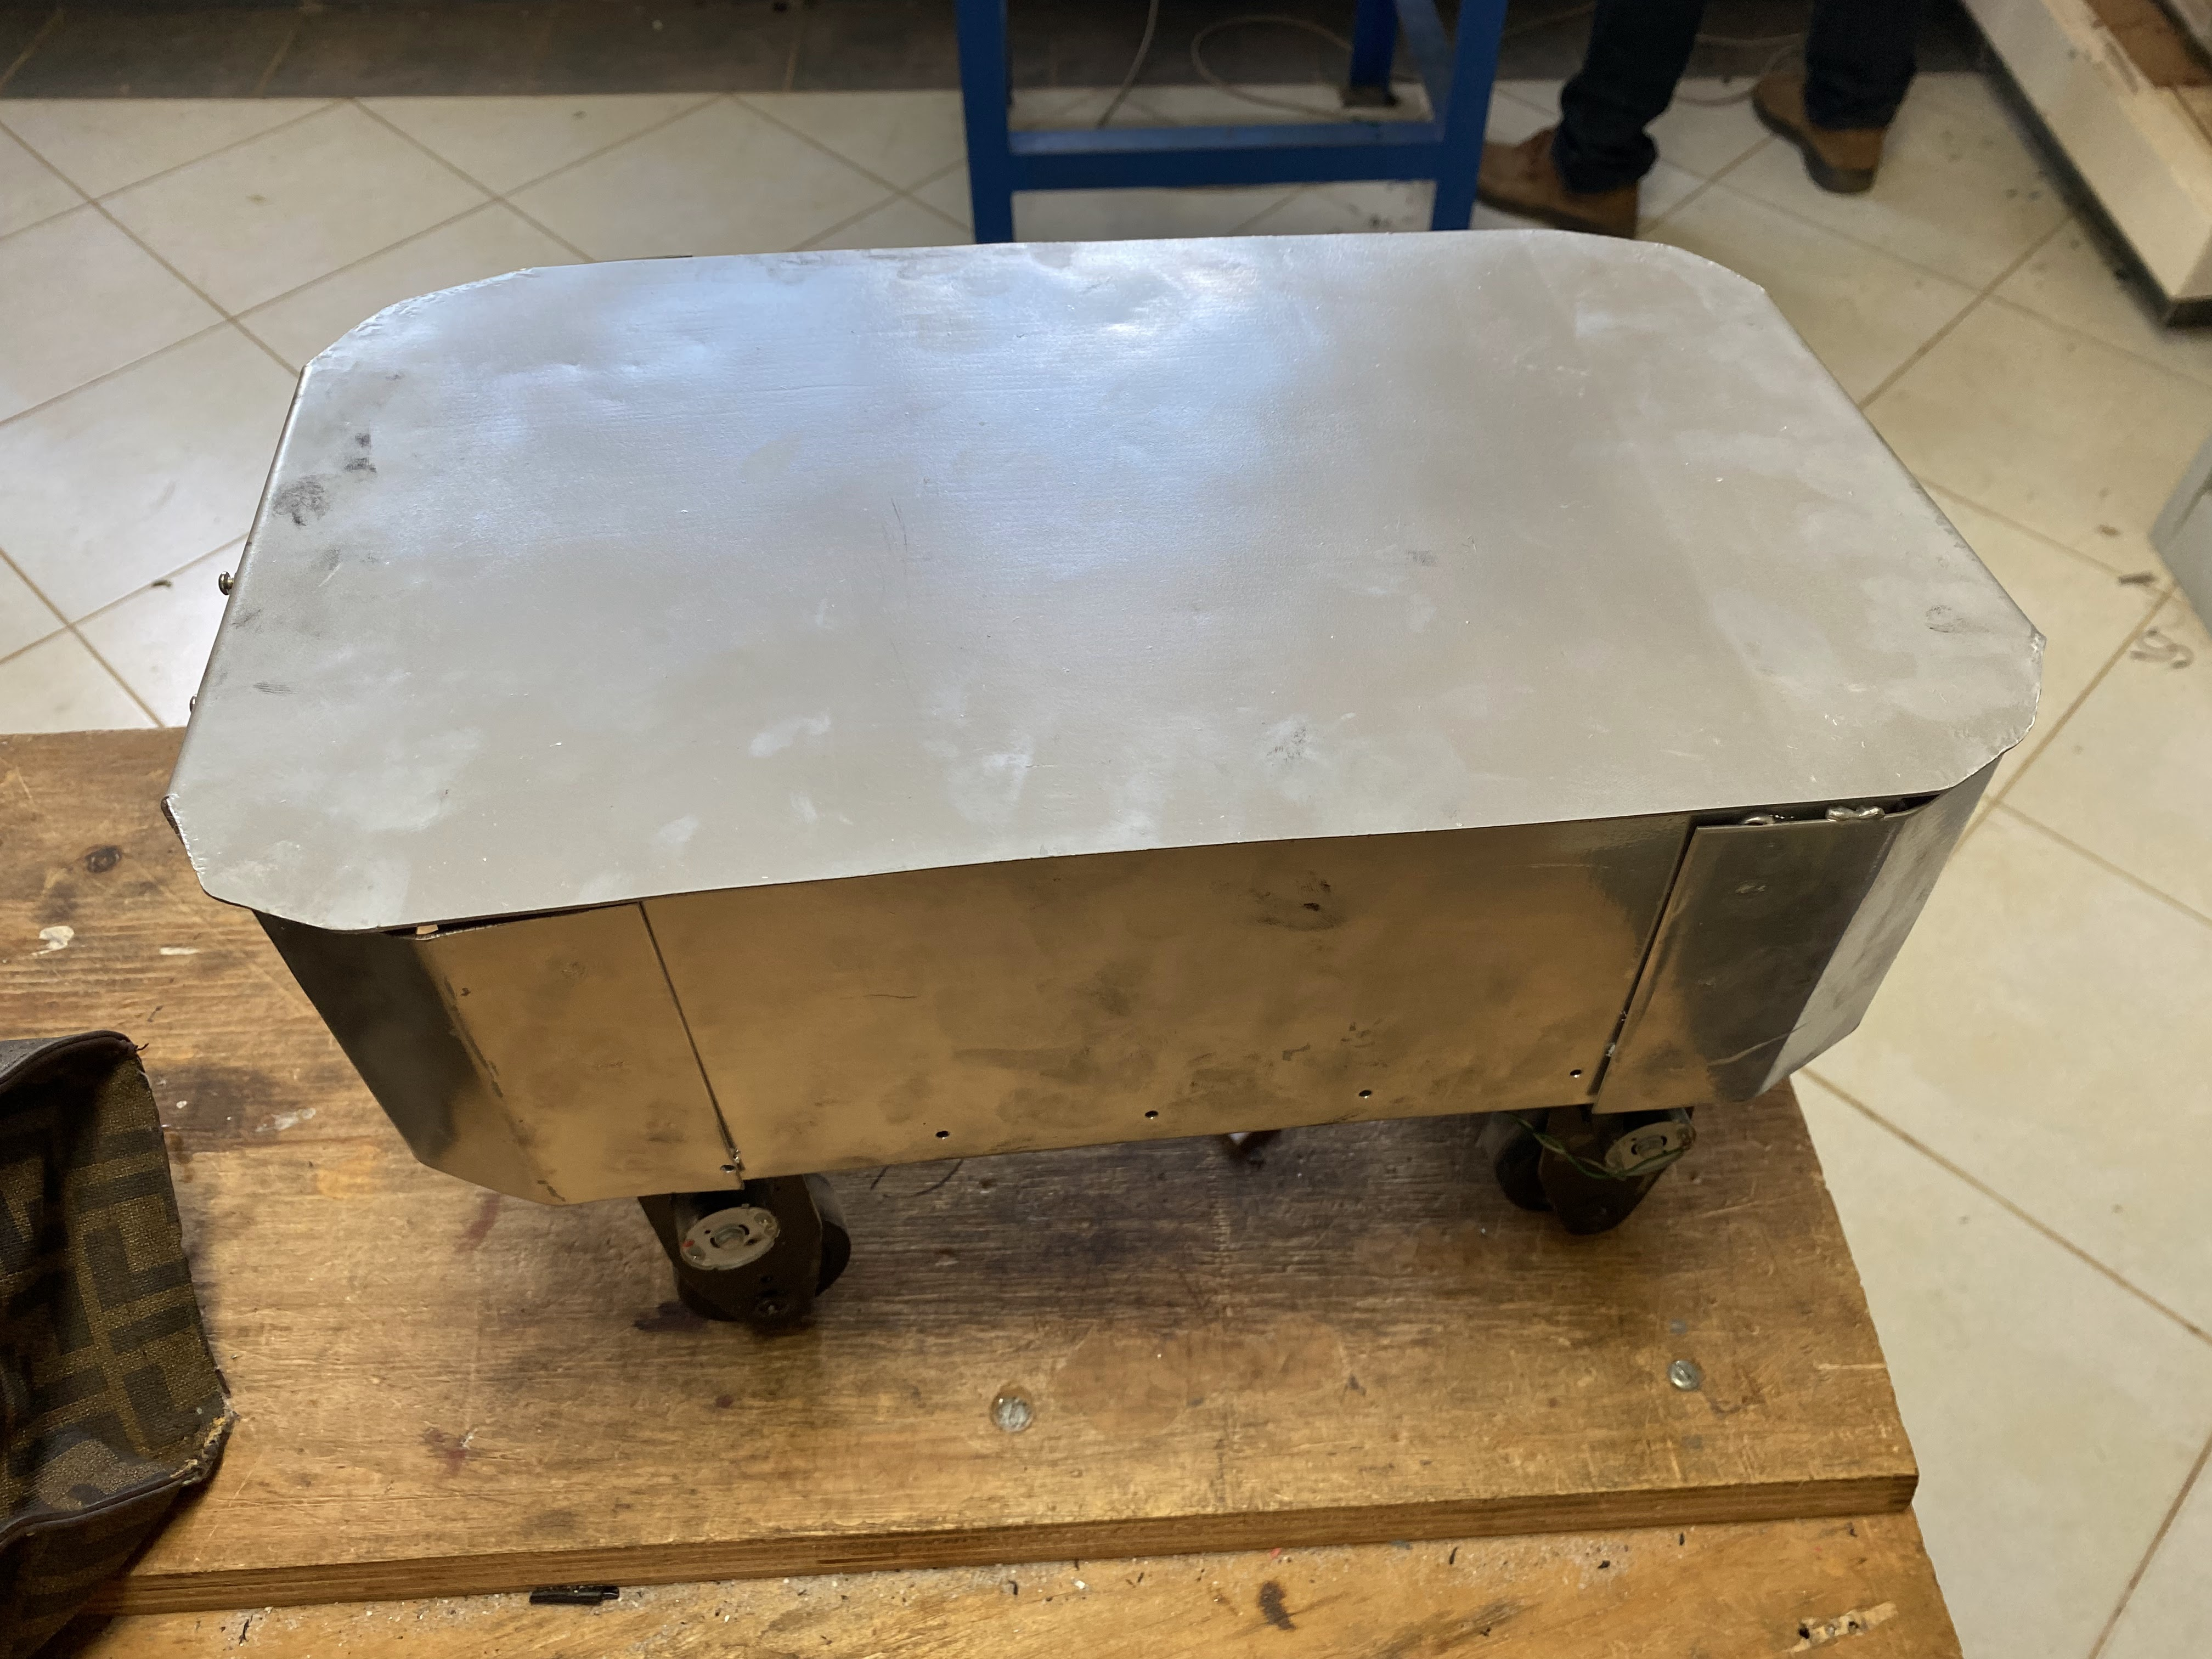
\includegraphics[scale = 0.08]{Figures/finalAssemblyCLOSED1.jpg}
    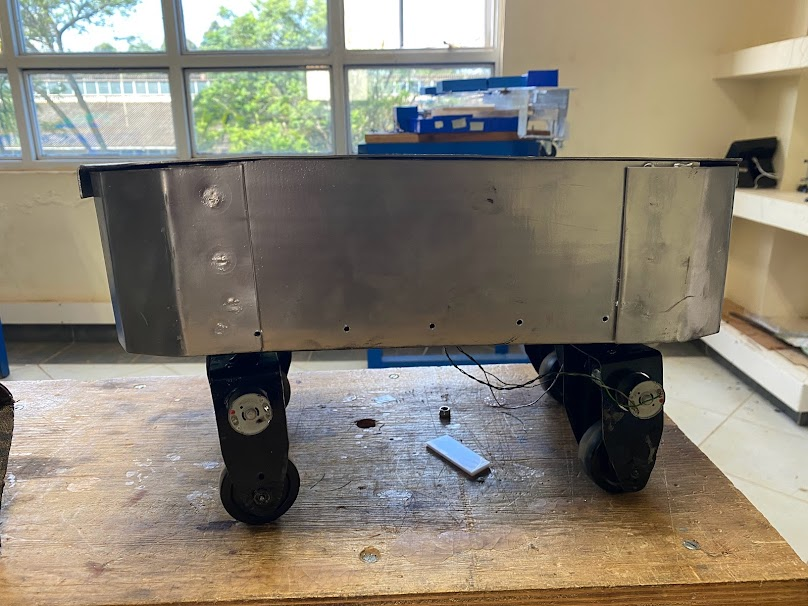
\includegraphics[scale = 0.4]{Figures/finalAssemblyCLOSED2.jpg}
    \caption{Fabricated Platform}
    \label{fig:fabassemblyplatform}
\end{figure}


After several experiments and tests, sending data between the mobile platform and the control clients (mobile application and hand motion control device) was confirmed. The data received by the mobile platform was for yaw and pitch values. This experiment was conducted by simulating \ac{PWM} signals on an oscilloscope as shown in Figure \ref{fig:pwmResult}, signals that would control the \ac{DC} motor speed.

\begin{figure}[H]
    \centering
    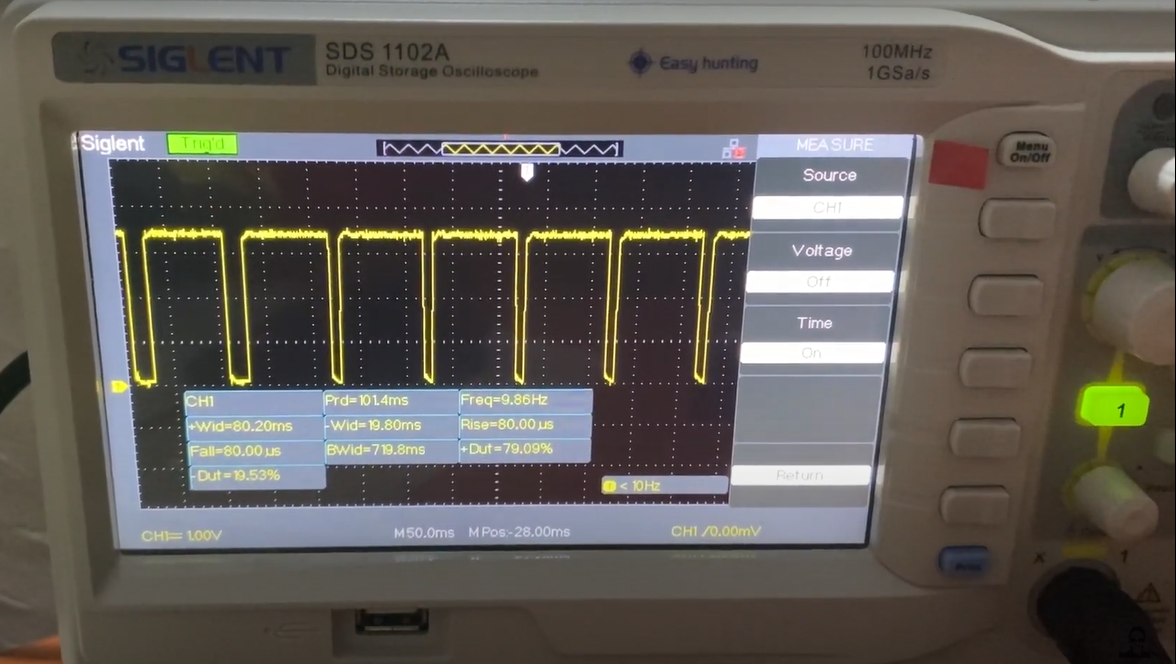
\includegraphics[scale = 0.4]{Figures/pwmResults.png}
    \caption{PWM Signals Generated using Transmitted Data}
    \label{fig:pwmResult}
\end{figure}

\par
Once data transmission was simulated, the next step was driving the mobile platform remotely. To do this, a pre-defined trajectory was determined in order to test the orientation and stability of the mobile platform. The platform followed the path as expected but veered off the path a few times due to misalignment arising from the fabrication process. The trajectory path was set up to ensure omnidirectional and holonomic movements could be achieved. The path is shown in Figure \ref{fig:desiredPath} and the resultant path followed by the mobile platform is shown in Figure \ref{fig:actualpath}. The comparison between desired path and actual path is shown in Figure \ref{fig:desiredandactualmotion}

\begin{figure}[H]
    \centering
    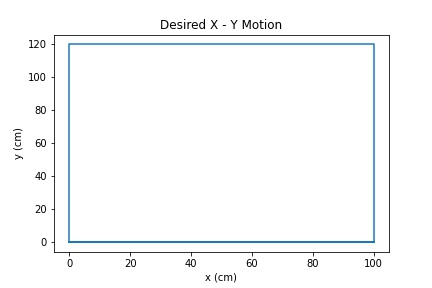
\includegraphics[scale = 0.8]{Figures/desiredmotion.jpeg}
    \caption{Desired Path}
    \label{fig:desiredPath}
\end{figure}

\begin{figure}[H]
    \centering
    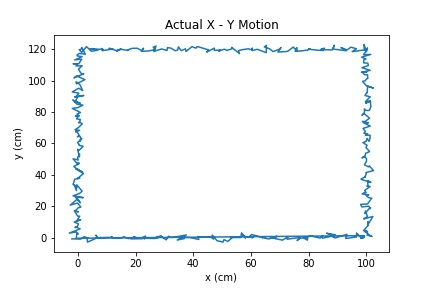
\includegraphics[scale = 0.8]{Figures/actualmotion.jpeg}
    \caption{Actual Path}
    \label{fig:actualpath}
\end{figure}

\begin{figure}[H]
    \centering
    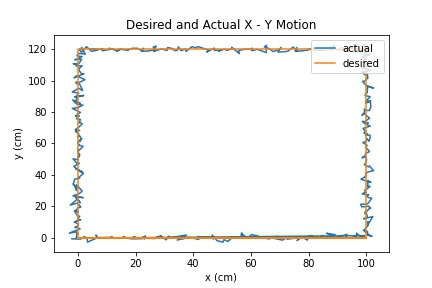
\includegraphics[scale = 0.8]{Figures/desiredandactualmotion.jpeg}
    \caption{Desired and Actual Path}
    \label{fig:desiredandactualmotion}
\end{figure}

From the Figure \ref{fig:desiredandactualmotion} it it clear the platform is able to achieve holonomic and omnidirectional motion. With a little bit of tuning to reduce the misalignment, the platform can be able to move in the desired trajectory.

\par
Other parameters, such as time to run vs velocity of the platform was measured and recorded in Table \ref{table:timetorunplatform}.

\begin{table}[ht]
  \begin{center}
    \leavevmode
    \hangcaption[Time and Acceleration under Different Payloads]{Time and Acceleration under Different Payloads}  
    \label{table:timetorunplatform}
\begin{tabular}{ |c|c| } 
 \hline
 Duration (min) & Velocity (m/s) \\ \hline 
 5 & 0.5 m/s \\ \hline
 10 & 0.5 m/s \\ \hline
 15 & 0.4 m/s \\ \hline
 20 & 0.3 m/s \\ \hline 
 25 & 0 m/s \\ \hline
\end{tabular}
\label{table:timetorunplatform}
  \end{center}
\end{table}

From Table \ref{table:timetorunplatform}, we were not able to achieve the ${44 mins}$ duration we had planned to achieve. This is due to the factor that we purchased a stepper motor for directional motion rather than a DC motor which consumes more power.

\subsection{Discussion}

The results of the design and fabrication of the prototype mobile platform with holonomic and omnidirectional motion are as follows:

\begin{enumerate}
    \item The mobile platform was tested in various scenarios, including moving in straight lines, turning, and moving in circular paths. It was found that the platform was not able to move smoothly and accurately in any direction, with the speed and direction being easily controlled using the mobile application and hand motion control device.
    \item The mobile platform was able to carry a payload of up to 10kg without any issues, demonstrating its versatility and potential use in various applications such as material handling and transportation.
    \item The mobile platform was found to be energy efficient, with the DC motors consuming minimal power even when operating at high speeds.    
\end{enumerate}


Overall, the results of this project show that it is possible to design and fabricate a prototype mobile platform with holonomic and omnidirectional motion using caster wheels and motors, and that this type of platform has the potential for various applications in the industry. The results showcased, show that the mobile platform was fabricated to a large extent as conceived in the design process. Furthermore, transmission of data between the clients through the channel as envisioned in Section \ref{sec:remoteClients} was achieved as proven by the generation of PWM signals which drive the DC motors in Figure \ref{fig:pwmResult}.
\par
This data was used to drive the mobile platform along a predetermined path but from Figure \ref{fig:desiredandactualmotion}, it was clear that there were misalignments that interfered with the velocity and ultimately the orientation of the mobile platform. These misalignments came about when the wheel frame in Figure \ref{fig:frameFAB} was being bent using the manual bending machine. A lot of estimations had to be made during the metal sheet bending process, which ultimately made the final product less like the design.

